\documentclass[10pt]{article}
\usepackage[pdftex]{graphicx}
\graphicspath{{./images/}}
\usepackage{amsmath,amssymb}
\usepackage{dirtytalk}
\usepackage{anyfontsize}
\usepackage{xcolor}
\usepackage{hyperref}
\hypersetup{
    colorlinks,
    linkcolor={red!50!black},
    citecolor={blue!50!black},
    urlcolor={blue!80!black}
}
\usepackage[skip=10pt plus1pt, indent=40pt]{parskip}
\usepackage{../../common_styles/csagh}


\begin{document}
\begin{opening}
  \title{K-Nearest-Neighbor with Python}
  \author[Universidad Autónoma de Nuevo León, San Nicolás de los Garza, aldo.hernandezt@uanl.edu.mx]{Aldo Hernández}

  \keywords{...}
  \begin{abstract}
    This document examines the implementation of K-Nearest Neighbor (KNN) classification for sentiment analysis of app reviews. Using a dataset of 257 user reviews, we demonstrate how a nonparametric KNN model can effectively predict star ratings based on word count and sentiment value features. After normalizing the data and determining the optimal k-value through empirical testing, our model achieved 83.1\% accuracy with a macro average f1-score of 0.81. The study illustrates the practical application of instance-based learning techniques in sentiment analysis tasks and discusses the theoretical foundations of distance metrics in KNN algorithms. Our visualization of the classification regions demonstrates how this approach effectively separates different rating categories in a two-dimensional feature space, providing an intuitive understanding of the model's decision boundaries.
  \end{abstract}

  \keywords{k-nearest-neighbor, python, classification, machine learning}
\end{opening}

\section{Introduction}
Nearest neighbor is a \textbf{nonparametric model}, it cannot be characterized by a bounded set of parameters \cite{ai}. For example, suppose an hypothesis that when generated, retains within itslef all of the training examples and uses them to predict the next example. This hypothesis would be nonparametric since the number of parameters is not bounded, as it grows with the number of examples. This approach is called \textbf{instance-based learning} \cite{ai}. \par
The simplest method for instance-based learning is \textbf{table lookup}, where when asked for $h(x)$, see if $x$ is in a table with all the training examples; if it is, return the corresponding $y$, if not, return a default value \cite{ai}. Table lookup can be improved by doing a slight variation: given a query $x_{q}$, find the $k$ examples nearest to $x_{q}$. This variation is what is known as \textbf{k-nearest neighbors} lookup, where the $k$ nearest neighbors are denoted by $NN(k, x_{q})$. \par
To perform classification using this supervised method, we first have to find $NN(k, x_{q})$, then take the plurality vote of the neighbors. To avoid ties, $k$ is always chosen to be an odd number. In the other side, to do regression we can take the mean or median of all neighbors, or solve a linear regression problem on the neighbors. \par
The name of the method implies that we need a way to measure distance---a metric---. How would we measure the distance from a query point $x_{q}$ to an example point $x_{j}$? Usually, these distances are calculated with a \textbf{Minkowski distance} (also called a $L^{p}$ norm), defined as
\begin{equation*}
    L^{p}(x_{j}, x_{q}) = \left(\sum_{i}\left|x_{j, i} - x_{q, i}\right|^{p}\right)^{1/p}
\end{equation*}
We can see that with $p = 2$ the norm is Euclidean distance and with $p = 1$ it is Manhattan distance. When using Boolean attribute values, the number of attributes on which two points differ is called the \textbf{Hamming distance} \cite{ai}. Euclidean distance is usually used when dimensions are measuring similar properties (like width, height, depth, etc.), while Manhattan distance is used if they are dissimilar (such as age, gender, weight, etc.). \par
It is important to note that if we use the raw numbers from each dimension then the total distance will be affected by a change in scale in any dimension, to avoid this, it is common to apply \textbf{normalization} to the measurements in each dimension, such that all $x_{j, i}$ becomes $(x_{j, i} - \mu_{i}) / \sigma_{i}$. Though there are other alternatives like the \textbf{Mahalanobis distance}, that takes into account the covariance between dimensions. \par
In low-dimensional spaces with a lot of data, nearest neighbors works very well since we are likely to have enough nearby data points to get a good answer \cite{ai}. But as we add dimensions, nearest neighbors in high-dimensional spaces are usually not very near. To imagine this, consider k-nearest-neighbors on a dataset of $N$ points uniformly distributed throughout the interior of an $n$-dimensional unit hypercube. We define the k-neighborhood of a point as the smallest hypercube that contains the k-nearest neighbors. Let $L$ be the average side length of a neighborhood. Then the volume of the neighborhood is $L^{n}$ and the volume of the full cube is 1. So, on average, $L = (k/N)^{1/n}$; now, let $k = 10$ and $N = 1,000,000$. If $n=2$, the average neighbourhood has $L=0.003$, but if $n=200$ then it is $L \approx 0.94$. This problem is known as the \textbf{curse of dimensionality} \cite{ai}. \par
The $NN(k, x_{q})$ function is conceptually simple: given a set of $N$ examples and a query $x_{q}$, iterate through the examples, then measure the distance to $x_{q}$ from each one, and keep the best $k$ \cite{ai}. The downside of this approach is that it takes $O(N)$ execution time, but this algorithm can be enhanced with binary trees for a $O(\log N)$ time or a hash table for a $O(1)$ time.

\section{Methodology}
\subsection{Before typing any code}
First, we have to download our dataset that is contained in a \href{http://www.aprendemachinelearning.com/wp-content/uploads/2018/07/reviews_sentiment.csv}{.csv file}. This dataset contains 257 user opinions about an app (reviews). Our inputs will be only two columns for the sake of graphing in 2D: word count and sentiment value. The output tags will be the stars given by the users to the app. Now, we import the necessary libraries
\begin{figure}[h]
    \centering
    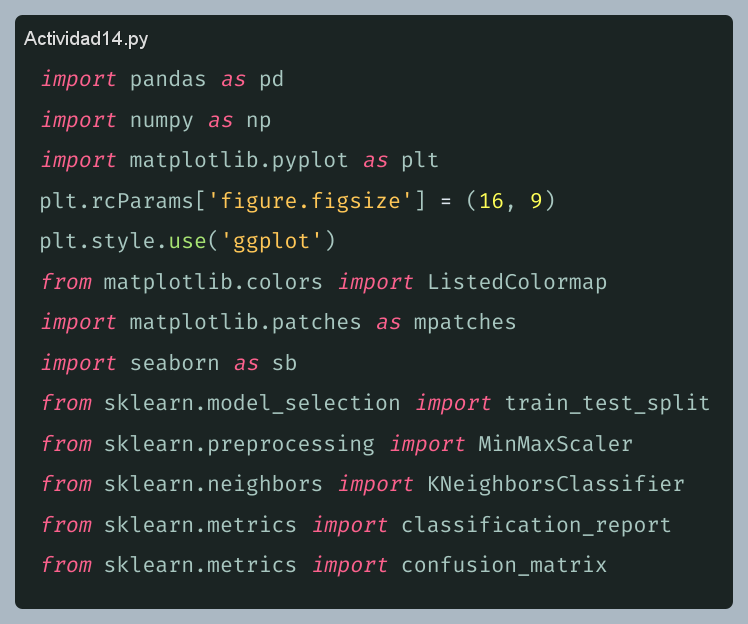
\includegraphics[width=90mm]{2025-03-31-17-28-34.png}
    \caption{Importing the essential libraries.}
\end{figure}

\subsection{Data visualization}
We can see that our dataset contains 257 rows along 7 columns, also around the 66\% of the dataset has their word count around $11.5 \pm 13.16$, their sentiment value around $0.38 \pm 0.90$, and their star rating around $3.42 \pm 1.41$. This means that the vast majority of reviews have from 0 to 24 words, the majority are positive reviews, and the rating is usually from 2 to 5 stars. We can also notice that the most popular ratings are 3 and 5 stars, as shown in the following figure
\begin{figure}[h]
    \centering
    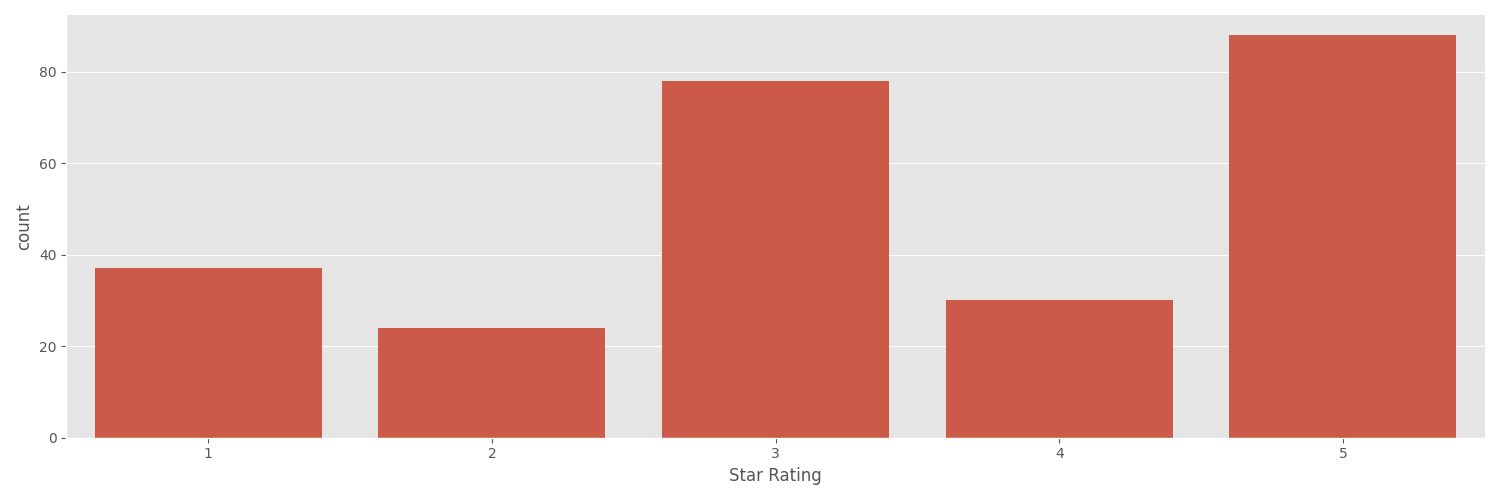
\includegraphics[width=130mm]{star_rating.png}
    \caption{Star ratings vs count.}
\end{figure}

\subsection{Preparing the data}
Next, we split our data into a training set and a test set. Then, we \textit{normalize} the data using a scaler.
\begin{figure}[h]
    \centering
    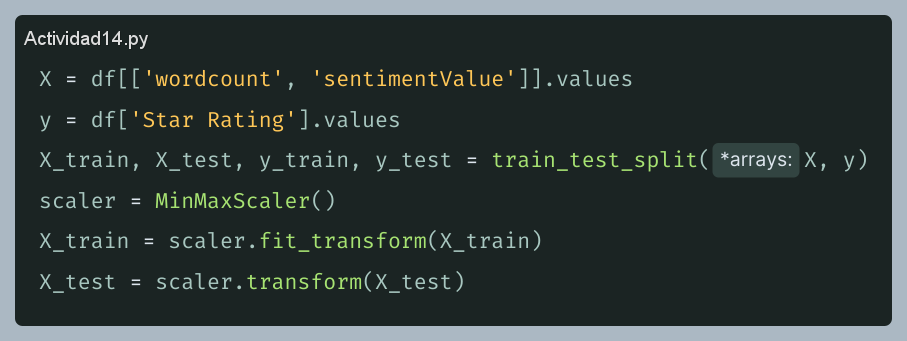
\includegraphics[width=90mm]{2025-03-31-17-42-05.png}
    \caption{Normalizing the data.}
\end{figure}

\newpage
Now, we have to figure out which $k$-value are we going to use. To do this, we can use the following code to get an idea of the best possible values \par
\begin{figure}[h]
    \centering
    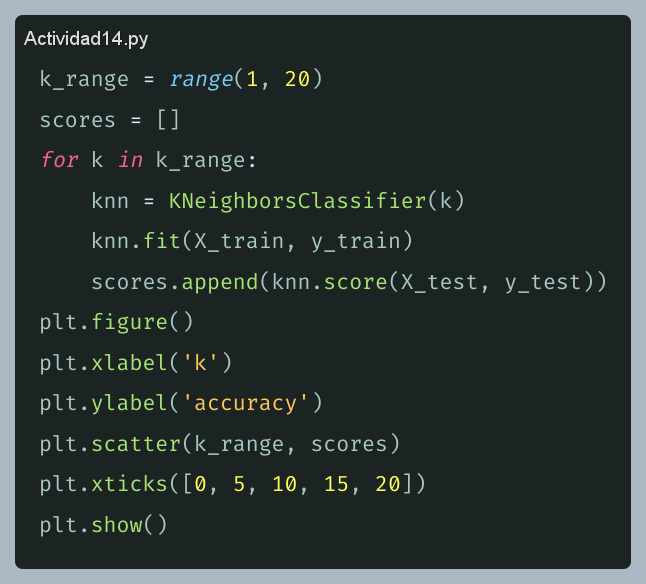
\includegraphics[width=70mm]{2025-03-31-17-48-31.png}
    \caption{Iterating through the possible $k$ values.}
\end{figure}
Usually, the optimal $k$ will be 3, 5 or 7 (for this dataset). We decided to pick $k=7$.

\subsection{Creating the model}
The next thing that we are going to do is to create the model. When testing it with test data, we get a 83.1\% of accuracy, which is a pretty good score. We can see that we got a macro average f1-score of 0.81 which is also a good indicator, in the confusion matrix we observe that the model only got wrong 11 predictions.
\begin{figure}[h]
    \centering
    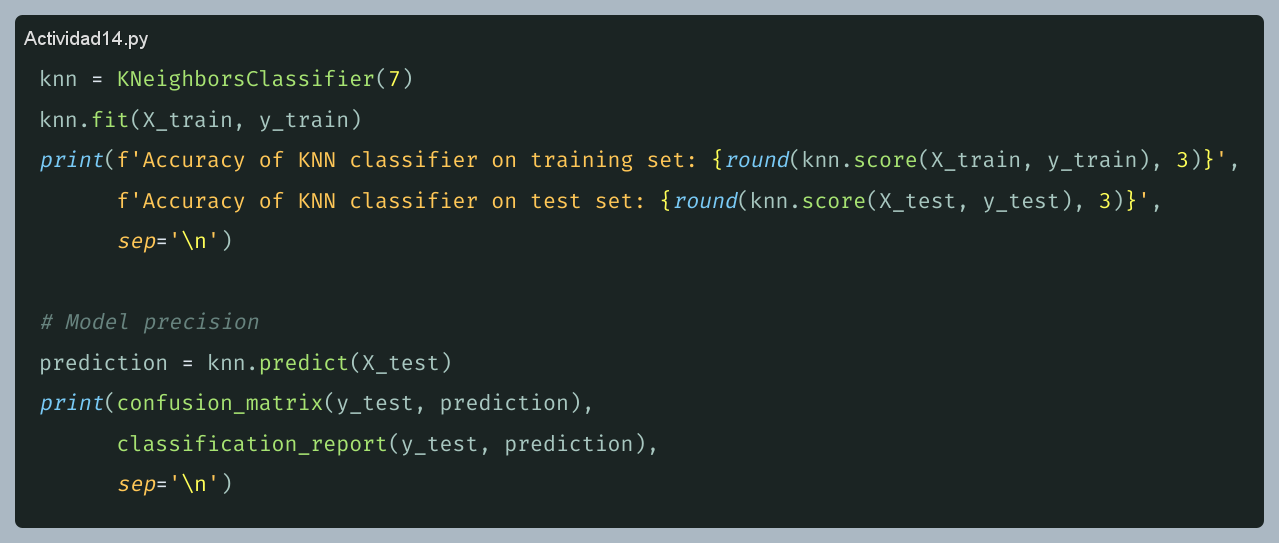
\includegraphics[width=100mm]{2025-03-31-17-57-05.png}
    \caption{Creating the KNN Classifier model.}
\end{figure}

\subsection{Plotting the graph}
Finally, we are all set to make the graph of our model. This graph will show the 5 different regions for classification along a 2-dimensional space based on the sentiment value (y-axis) and word count (x-axis), as shown
\begin{figure}[h]
    \centering
    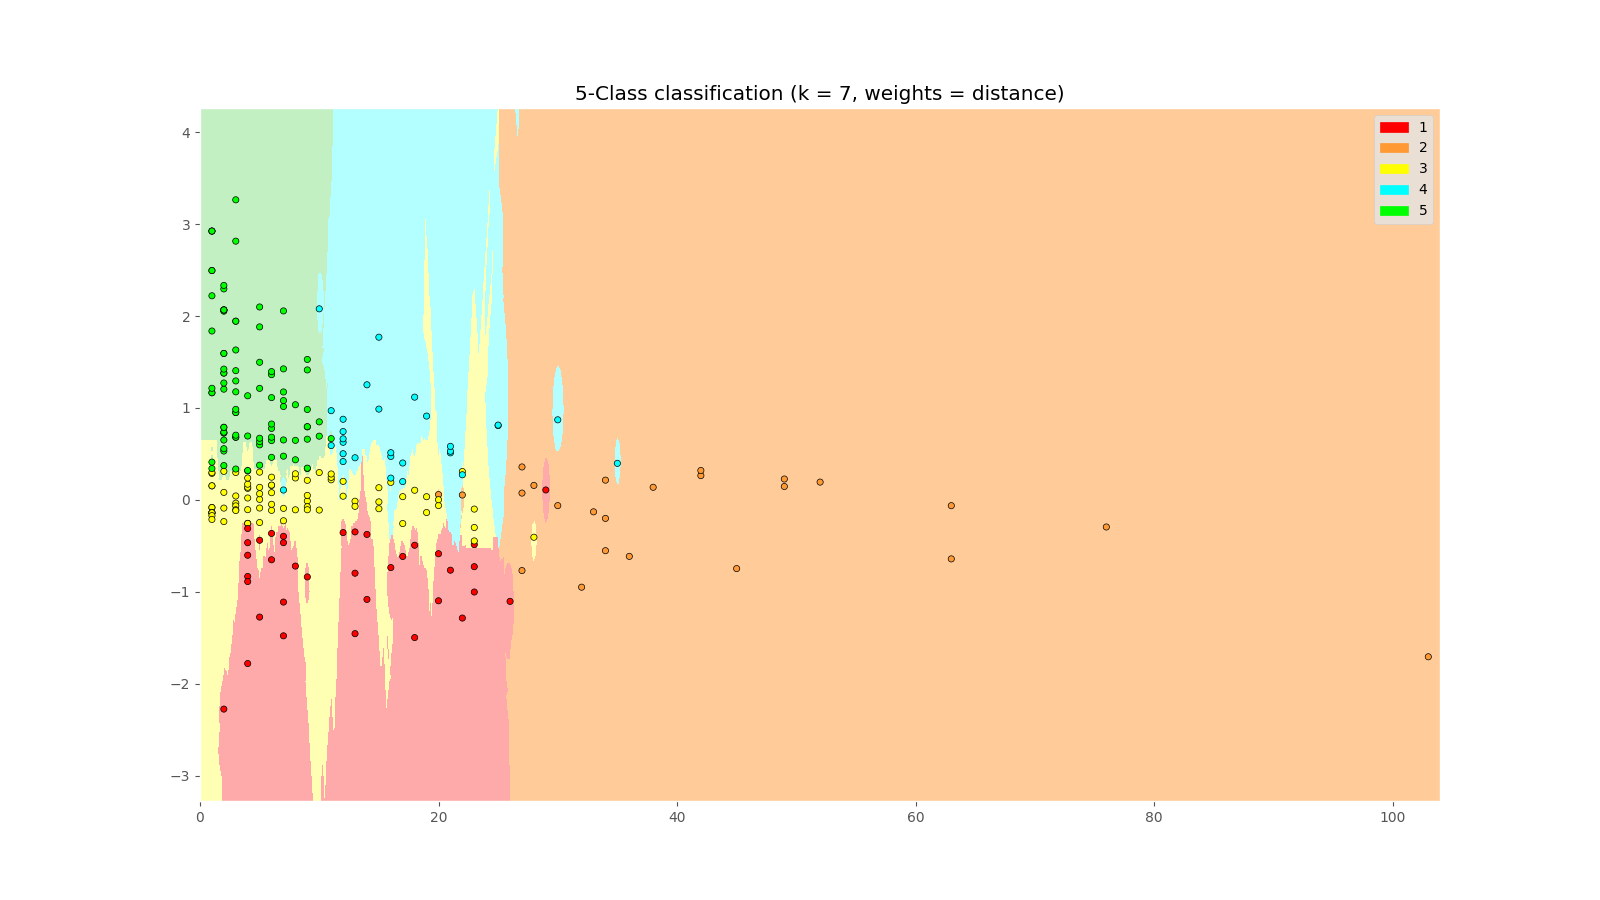
\includegraphics[width=130mm]{color_graph_k7.png}
    \caption{All regions for classification.}
\end{figure}

\section{Results}
With this model, we can finally predict the star rating of a review. For example, let's suppose we have a review with 5 words and 1 sentiment value, then the model predicts that the review has a rating of 5 stars with a 92.04\% of reliability.

\section{Conclusions}
The K-Nearest Neighbor approach demonstrated significant effectiveness in predicting star ratings from user reviews based solely on word count and sentiment value. With an accuracy of 83.1\% and a macro average f1-score of 0.81, the model proved capable of distinguishing between different rating categories despite the simplicity of the features used. This success highlights the power of nonparametric, instance-based learning methods for classification tasks when properly implemented. \par
The visualization of classification regions clearly illustrates how the model partitions the feature space, providing valuable insights into the relationship between textual characteristics and user satisfaction levels. The model's high reliability in predicting extreme ratings (particularly 5-star reviews) suggests that sentiment value is especially indicative of user satisfaction. \par
While our implementation used only two features for visualization purposes, the KNN algorithm could potentially achieve even higher accuracy by incorporating additional textual features. Future work might explore methods to address the curse of dimensionality when using larger feature sets and investigate performance optimizations through tree-based or hashing techniques as mentioned in the theoretical background. \par
Overall, this implementation demonstrates that KNN is not only conceptually straightforward but also practically effective for sentiment analysis tasks, confirming its value as a baseline approach for classification problems in natural language processing applications.

\bibliographystyle{../common_styles/cs-agh}
\bibliography{act14_bibliography}

\end{document}